\documentclass[twocolumn]{article}

\usepackage[utf8]{inputenc}
\usepackage{CJKutf8}
\usepackage{CJK}
\usepackage{amsmath}
\usepackage{amsthm}
\usepackage{amssymb}
\usepackage{newfloat}
\usepackage{setspace}
\usepackage{tikz}
\usepackage{fancyhdr}
\allowdisplaybreaks[4]
\usetikzlibrary{arrows,graphs}
\usetikzlibrary{graphs}
\usetikzlibrary{graphs.standard}
\newenvironment{SChinese}{%
	\CJKfamily{gbsn}%
	\CJKtilde
	\CJKnospace}{}
\pagestyle{fancy}
\fancyhead[L]{Problem Solving III}
\begin{document}
	\begin{CJK}{UTF8}{}	
		\begin{SChinese}	
			\title{问题求解(三)第6周作业}
			\author{黄奕诚 161220049}
			\maketitle
			
			\section*{8.1}
			\subsection*{(a)}
				对于$u_0$,非平凡完全图边数可以为$1(n=2),3(n=3),6(n=4 )$;对于$u_1$,树上任意两顶点之间只有唯一路径,否则会成圈,不满足树的性质;对于$u_2$,可迁竞赛图不含圈,故答案为0;对于$u_3$,6阶树含有5条边,由于不含圈,故每条边都是割边;对于$u_4$,7阶非空正则图的$r$可以是2~7之间的偶数,即2,4,6;对于$u_5$,通过穷举,容易得出5阶树的最大度可以为2,3,4;对于$u_6$,5阶图当形如一条折线时,有最大割点个数,为3;\\
				综上所述:
				\begin{center}
					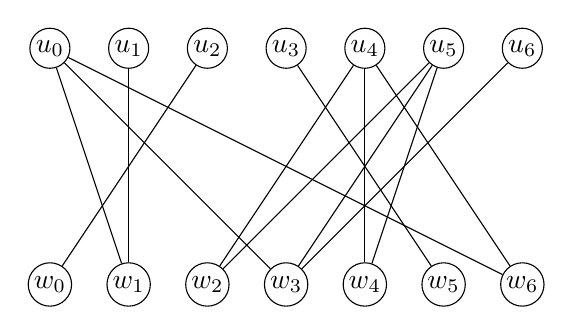
\begin{tikzpicture}
					\tikzstyle{vertex}=[circle,draw=black,minimum size=5pt,inner sep=1pt]
					\node[vertex] (1) at (0,0) {$u_0$};
					\node[vertex] (2) at (1,0) {$u_1$};
					\node[vertex] (3) at (2,0) {$u_2$};
					\node[vertex] (4) at (3,0) {$u_3$};
					\node[vertex] (5) at (4,0) {$u_4$};
					\node[vertex] (6) at (5,0) {$u_5$};
					\node[vertex] (7) at (6,0) {$u_6$};
					\node[vertex] (8) at (0,-3) {$w_0$};
					\node[vertex] (9) at (1,-3) {$w_1$};
					\node[vertex] (10) at (2,-3) {$w_2$};
					\node[vertex] (11) at (3,-3) {$w_3$};
					\node[vertex] (12) at (4,-3) {$w_4$};
					\node[vertex] (13) at (5,-3) {$w_5$};
					\node[vertex] (14) at (6,-3) {$w_6$};
					\draw (1) -- (9);
					\draw (1) -- (11);
					\draw (1) -- (14);
					\draw (2) -- (9);
					\draw (3) -- (8);
					\draw (4) -- (13);
					\draw (5) -- (10);
					\draw (5) -- (12);
					\draw (5) -- (14);
					\draw (6) -- (10);
					\draw (6) -- (11);
					\draw (6) -- (12);
					\draw (7) -- (11);
					\end{tikzpicture}
				\end{center}
			\subsection*{(b)}
				包含完美匹配,如下图所示:
				\begin{center}
					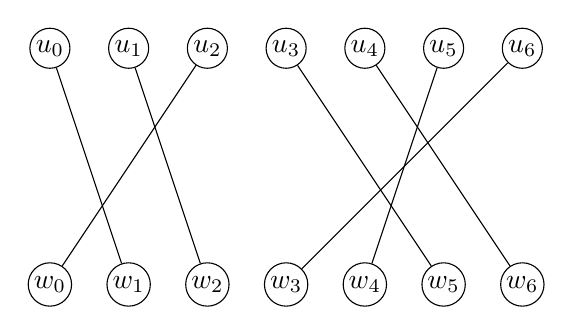
\begin{tikzpicture}
					\tikzstyle{vertex}=[circle,draw=black,minimum size=5pt,inner sep=1pt]
					\node[vertex] (1) at (0,0) {$u_0$};
					\node[vertex] (2) at (1,0) {$u_1$};
					\node[vertex] (3) at (2,0) {$u_2$};
					\node[vertex] (4) at (3,0) {$u_3$};
					\node[vertex] (5) at (4,0) {$u_4$};
					\node[vertex] (6) at (5,0) {$u_5$};
					\node[vertex] (7) at (6,0) {$u_6$};
					\node[vertex] (8) at (0,-3) {$w_0$};
					\node[vertex] (9) at (1,-3) {$w_1$};
					\node[vertex] (10) at (2,-3) {$w_2$};
					\node[vertex] (11) at (3,-3) {$w_3$};
					\node[vertex] (12) at (4,-3) {$w_4$};
					\node[vertex] (13) at (5,-3) {$w_5$};
					\node[vertex] (14) at (6,-3) {$w_6$};
					\draw (2) -- (10);
					\draw (3) -- (8);
					\draw (4) -- (13);
					\draw (7) -- (11);
					\draw (1) -- (9);
					\draw (5) -- (14);
					\draw (6) -- (12);
					\end{tikzpicture}
				\end{center}
			\section*{8.3}
			\subsection*{(a)}
				能够完美匹配(对任意的$X$有$|N(X)|\ge |X|$),如下图所示:
				\begin{center}
					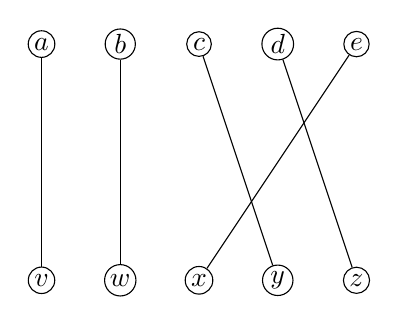
\begin{tikzpicture}
					\tikzstyle{vertex}=[circle,draw=black,minimum size=5pt,inner sep=1pt]
					\node[vertex] (1) at (0,0) {$a$};
					\node[vertex] (2) at (1,0) {$b$};
					\node[vertex] (3) at (2,0) {$c$};
					\node[vertex] (4) at (3,0) {$d$};
					\node[vertex] (5) at (4,0) {$e$};
					\node[vertex] (6) at (0,-3) {$v$};
					\node[vertex] (7) at (1,-3) {$w$};
					\node[vertex] (8) at (2,-3) {$x$};
					\node[vertex] (9) at (3,-3) {$y$};
					\node[vertex] (10) at (4,-3) {$z$};
					\draw (1) -- (6);
					\draw (2) -- (7);
					\draw (3) -- (9);
					\draw (4) -- (10);
					\draw (5) -- (8);
					\end{tikzpicture}
				\end{center}
			\subsection*{(b)}
			  不能完美匹配,因为存在$X=\{v,x,y\},N(X)=\{a,c\}$,此时$|X|>|N(X)|$,如此不能完美匹配.
			\section*{8.4}
				\begin{proof}
					由于有条件$|U|=|W|=k\ge2$,且$U$中任意两点在$G$中有不同的度,不妨设$\textrm{Degree}(u_1)=1,\textrm {Degree}(u_2)=2,\cdots,\textrm{Degree}(u_k)=k$,如此对$U$中任意子集$X$,设$X$中最大下标为$t$,则有$|N(X)|\ge t\ge|X|$,因此满足完美匹配.
				\end{proof}
			\section*{9.6}
				\subsection*{(a)}
					\textbf{正确}
					\begin{proof}
						平面图可以构成在平面内任意两条边都不相交的平图,此时去掉任意的边或顶点,仍然满足任意两条边都不相交的性质,因此平面图的子图仍是平面图.
					\end{proof}
				\subsection*{(b)}
					\textbf{错误}
					\begin{proof}
						非平面图的顶点个数必大于等于4,只要取其中一条边作为它的子图即可,显然是平面图,故命题不成立.
					\end{proof}
				\subsection*{(c)}
					\textbf{错误}
					\begin{proof}
						反例:对于$K_{3,3}$来说,任意删去一条边,则
						\begin{center}
							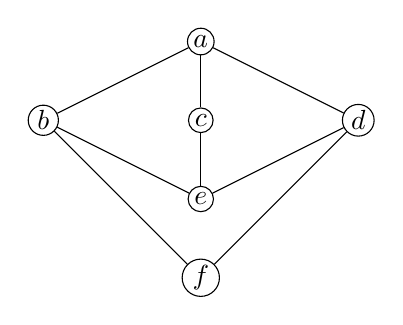
\begin{tikzpicture}
							\tikzstyle{vertex}=[circle,draw=black,minimum size=5pt,inner sep=1pt]
							\node[vertex] (1) at (0,0) {$a$};
							\node[vertex] (2) at (-2,-1) {$b$};
							\node[vertex] (3) at (0,-1) {$c$};
							\node[vertex] (4) at (2,-1) {$d$};
							\node[vertex] (5) at (0,-2) {$e$};
							\node[vertex] (6) at (0,-3) {$f$};
							\draw (1) -- (2);
							\draw (1) -- (3);
							\draw (1) -- (4);
							\draw (5) -- (2);
							\draw (5) -- (3);
							\draw (5) -- (4);
							\draw (6) -- (2);
							\draw (6) -- (4);
							\end{tikzpicture}
						\end{center}
					\end{proof}
					此时为平面图.
				\subsection*{(d)}
					\textbf{错误}
					\begin{proof}
						假若$G$包含$K_5$或$k_{3,3}$的细分作为子图,则不是平面图(由Theorem9.7可直接得到).
					\end{proof}
				\subsection*{(e)}
					\textbf{错误}
					\begin{proof}
						反例:$K_{3,3}$满足$n=6,m=9$,且$m\le 3n-6$,而它是非平面图.
					\end{proof}
				\subsection*{(f)}
					\textbf{错误}
					\begin{proof}
						反例:$K_{3,3}$在任意两个不相邻的顶点之间添加一条边,此时它具有三角形圈,但它存在$K_{3,3}$子图,因此不是平面图.
					\end{proof}
			\section*{9.13}
				\subsection*{(a)}
					\begin{proof}
						因为连通图$G$的顶点个数大于等于3,且边不构成三角形.当$n=3$时,$m=2$,满足$m\le 2n-4$.当$n=4$时,$m=3$或$m=4$,也满足$m\le 2n-4$.当$n\ge5$时,每个区域所包含的边至少有4条,记$m_i$为区域$R_i$所包含的边的个数,则$m_i\ge4$,于是\begin{displaymath}
							M=\sum_{i=1}^{r}m_i\ge4r.
						\end{displaymath}
						在这个计数中,若边为割边,则$M$记了一次,若边不是割边,则$M$记了2次,因此$M\le2m$,于是有$4r\le M\le 2m$,所以$2r\le m$.\\
						又由欧拉定理知$n-m+r=2$,所以$4=2n-2m+2r\le 2n-2m+m=2n-m$,由此$m\le2n-4$.
					\end{proof}
				\subsection*{(b)}
					\begin{proof}
						$K_{3,3}$中不含有三角形,并且顶点个数大于3.由于$n=6,m=9$而$m>2n-4$,因此由(a)中的逆否命题可知$K_{3,3}$不是平面图.
					\end{proof}
				\subsection*{(c)}
					\textbf{Disprove}
					\begin{proof}
						反例:对于$K_{3,3}$来说,任意删去一条边,则
						\begin{center}
							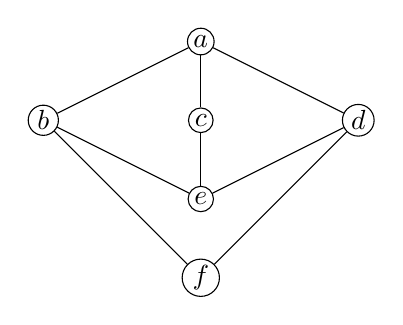
\begin{tikzpicture}
							\tikzstyle{vertex}=[circle,draw=black,minimum size=5pt,inner sep=1pt]
							\node[vertex] (1) at (0,0) {$a$};
							\node[vertex] (2) at (-2,-1) {$b$};
							\node[vertex] (3) at (0,-1) {$c$};
							\node[vertex] (4) at (2,-1) {$d$};
							\node[vertex] (5) at (0,-2) {$e$};
							\node[vertex] (6) at (0,-3) {$f$};
							\draw (1) -- (2);
							\draw (1) -- (3);
							\draw (1) -- (4);
							\draw (5) -- (2);
							\draw (5) -- (3);
							\draw (5) -- (4);
							\draw (6) -- (2);
							\draw (6) -- (4);
							\end{tikzpicture}
						\end{center}
						此时$G$的度数为6.
					\end{proof}
			\section*{9.14}
				\subsection*{(a)}	
					\begin{proof}
						因为连通图$G$的顶点个数大于等于5,且最小圈的长度为5,则每个区域所包含的边至少有5条,记$m_i$为区域$R_i$所包含的边的个数,则$m_i\ge5$,于是\begin{displaymath}
						M=\sum_{i=1}^{r}m_i\ge5r.
						\end{displaymath}
						在这个计数中,若边为割边,则$M$记了一次,若边不是割边,则$M$记了2次,因此$M\le2m$,于是有$5r\le M\le 2m$.\\
						又由欧拉定理知$n-m+r=2$,所以$20=10n-10m+10r\le 10n-10m+4m=2n-6m$,由此$m\le\frac{5}{3}(n-2)$.
					\end{proof}
				\subsection*{(b)}
					\begin{proof}
						因为Petersen图满足其边数最小的圈的边数为5,又$n=10,m=15$,而$m>\frac {5}{3}(n-2)$,因此Petersen图不是平面图.
					\end{proof}
				\subsection*{(c)}
					\begin{proof}
						Peterson图如图所示:
						\begin{center}
							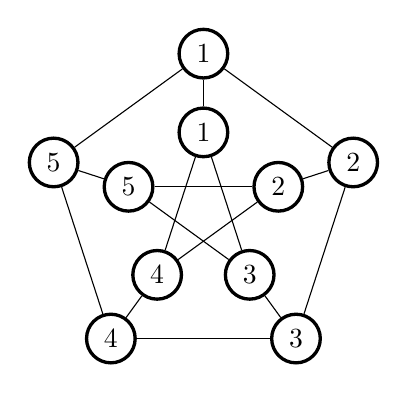
\begin{tikzpicture}[every node/.style={draw,circle,very thick}]
							\graph[clockwise, radius=2cm] {subgraph C_n [n=5,name=A]};
							\graph[clockwise, radius=1cm] {subgraph I_n [n=5,name=B]};
							
							\foreach \i in {1,2,3,4,5}{\draw (A \i) -- (B \i);}
							\newcounter{j}
							\foreach \i in {1,2,3,4,5}{%
								\pgfmathsetcounter{j}{ifthenelse(mod(\i+2,5),mod(\i+2,5),5)}
								\draw (B \i) -- (B \thej);
							}
							\end{tikzpicture}
						\end{center}
						(记内部5个顶点为$i_1,i_2,i_3,i_4,i_5$,外部5个顶点为$o_1,o_2,o_3,o_4,o_5$)\\
						下面找出其中包含的一个细分的$K_{3,3}$,即为
						\begin{center}
							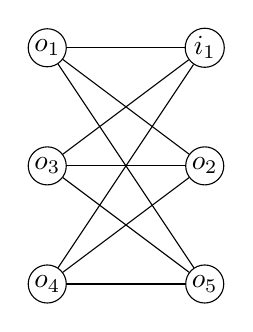
\begin{tikzpicture}
							\tikzstyle{vertex}=[circle,draw=black,minimum size=5pt,inner sep=1pt]
							\node[vertex] (1) at (0,0) {$o_1$};
							\node[vertex] (2) at (0,-1.5) {$o_3$};
							\node[vertex] (3) at (0,-3) {$o_4$};
							\node[vertex] (4) at (2,0) {$i_1$};
							\node[vertex] (5) at (2,-1.5) {$o_2$};
							\node[vertex] (6) at (2,-3) {$o_5$};
							\draw (1) -- (4);
							\draw (1) -- (5);
							\draw (1) -- (6);
							\draw (2) -- (4);
							\draw (2) -- (5);
							\draw (2) -- (6);
							\draw (3) -- (4);
							\draw (3) -- (5);
							\draw (3) -- (6);
							\end{tikzpicture}
						\end{center}
						因此由Kuratowski定理可知Petersen图不是平面图.
					\end{proof}
				\subsection*{(d)}
					\textbf{Disprove}
					\begin{proof}
						假设所有顶点的度数都大于等于3,则有$\sum_{i=1}^{n}(\textrm{degree})V_i\ge3n$,也即$2m\ge3n$.因为有$m\le\frac{5}{3}(n-2)$,故$3n\le\frac{10}{3}(n-2)$,得$n\ge20$,这与$n\le20$矛盾.因此存在度数小于等于2的顶点.
					\end{proof}
			\section*{9.15}
				\begin{proof}
					假设所有顶点的度数都大于等于5,则有$\sum_{i=1}^{n}(\textrm{degree})V_i\ge5n$,也即$2m\ge5n$.当$n=1,n=2$时矛盾,当$n\ge3$时,有$m\le3n-6$,故$5n\le6n-12$,得$n\ge12$,这与$n\le11$矛盾.因此存在度数小于等于4的顶点.
				\end{proof}
			\section*{10.1}
				对于$G_1$,存在奇圈,故$\chi(G_1)\ge3$,又存在如下图所示的染色数为3的情形:
				\begin{center}
					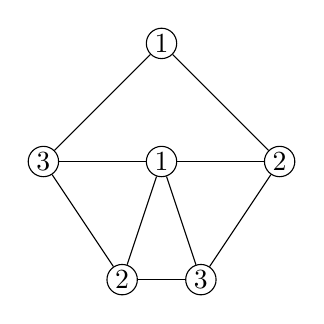
\begin{tikzpicture}
					\tikzstyle{vertex}=[circle,draw=black,minimum size=5pt,inner sep=1pt]
					\node[vertex] (1) at (0,0) {$1$};
					\node[vertex] (2) at (-1.5,-1.5) {$3$};
					\node[vertex] (3) at (0,-1.5) {$1$};
					\node[vertex] (4) at (1.5,-1.5) {$2$};
					\node[vertex] (5) at (-0.5,-3) {$2$};
					\node[vertex] (6) at (0.5,-3) {$3$};
					\draw (1) -- (2);
					\draw (1) -- (4);
					\draw (2) -- (3);
					\draw (3) -- (4);
					\draw (2) -- (5);
					\draw (3) -- (5);
					\draw (3) -- (6);
					\draw (4) -- (6);
					\draw (5) -- (6);
					\end{tikzpicture}
				\end{center}
				故$\chi(G_1)=3$.\\
				对于$G_2$,因为存在$K_4$子图,所以$\chi(G_2)\ge4$,又因为$G_2$是平面图,所以$\chi(G_2)\le4$,因此$\chi(G_2)=4$.\\
				对于$G_3$,存在$K_4$子图,所以$\chi(G_3)\ge4$,又存在如下图所示染色数为4的情形:
				\begin{center}
					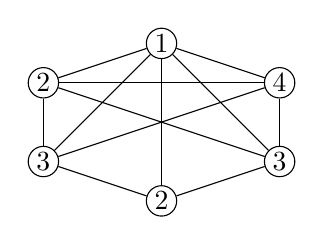
\begin{tikzpicture}
					\tikzstyle{vertex}=[circle,draw=black,minimum size=5pt,inner sep=1pt]
					\node[vertex] (1) at (0,0) {$1$};
					\node[vertex] (2) at (-1.5,-0.5) {$2$};
					\node[vertex] (3) at (1.5,-0.5) {$4$};
					\node[vertex] (4) at (-1.5,-1.5) {$3$};
					\node[vertex] (5) at (1.5,-1.5) {$3$};
					\node[vertex] (6) at (0,-2) {$2$};
					\draw (1) -- (2);
					\draw (1) -- (3);
					\draw (1) -- (4);
					\draw (1) -- (5);
					\draw (1) -- (6);
					\draw (2) -- (3);
					\draw (2) -- (4);
					\draw (2) -- (5);
					\draw (3) -- (4);
					\draw (3) -- (5);
					\draw (4) -- (6);
					\draw (5) -- (6);
					\end{tikzpicture}
				\end{center}
				故$\chi(G_3)=4$\\
				对于$G_4$,因为含有三角形,所以$\chi(G_4)\ge3$,又存在如下图所示的染色数为3的情形:
				\begin{center}
					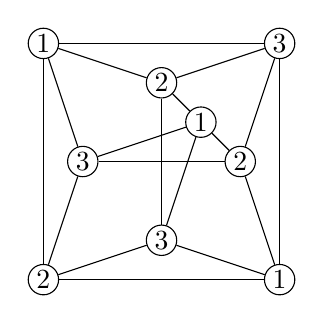
\begin{tikzpicture}
					\tikzstyle{vertex}=[circle,draw=black,minimum size=5pt,inner sep=1pt]
					\node[vertex] (1) at (0,0) {$1$};
					\node[vertex] (2) at (3,0) {$3$};
					\node[vertex] (3) at (1.5,-0.5) {$2$};
					\node[vertex] (4) at (0.5,-1.5) {$3$};
					\node[vertex] (5) at (2,-1) {$1$};
					\node[vertex] (6) at (2.5,-1.5) {$2$};
					\node[vertex] (7) at (0,-3) {$2$};
					\node[vertex] (8) at (1.5,-2.5) {$3$};
					\node[vertex] (9) at (3,-3) {$1$};
					\draw (1) -- (2);
					\draw (1) -- (3);
					\draw (1) -- (4);
					\draw (1) -- (7);
					\draw (2) -- (3);
					\draw (2) -- (6);
					\draw (2) -- (9);
					\draw (3) -- (5);
					\draw (3) -- (8);
					\draw (4) -- (5);
					\draw (4) -- (6);
					\draw (4) -- (7);
					\draw (5) -- (6);
					\draw (5) -- (8);
					\draw (6) -- (9);
					\draw (7) -- (8);
					\draw (7) -- (9);
					\draw (8) -- (9);
					\end{tikzpicture}
				\end{center}
				故$\chi(G_4)=3$.\\
				对于$G_5$,存在$K_4$为它的子图,因此$\chi(G_5)\ge4$,又存在如下图所示的染色数为4的情形:
				\begin{center}
					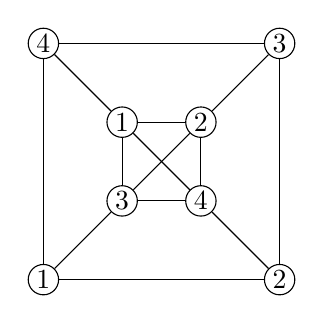
\begin{tikzpicture}
					\tikzstyle{vertex}=[circle,draw=black,minimum size=5pt,inner sep=1pt]
					\node[vertex] (1) at (0,0) {$4$};
					\node[vertex] (2) at (3,0) {$3$};
					\node[vertex] (3) at (0,-3) {$1$};
					\node[vertex] (4) at (3,-3) {$2$};
					\node[vertex] (5) at (1,-1) {$1$};
					\node[vertex] (6) at (2,-1) {$2$};
					\node[vertex] (7) at (1,-2) {$3$};
					\node[vertex] (8) at (2,-2) {$4$};
					\draw (1) -- (2);
					\draw (1) -- (3);
					\draw (1) -- (5);
					\draw (2) -- (4);
					\draw (2) -- (6);
					\draw (3) -- (4);
					\draw (3) -- (7);
					\draw (4) -- (8);
					\draw (5) -- (6);
					\draw (5) -- (7);
					\draw (5) -- (8);
					\draw (6) -- (7);
					\draw (6) -- (8);
					\draw (7) -- (8);
					\end{tikzpicture}
				\end{center}
				故$\chi(G_5)=4$.
			\section*{10.4}
				\subsection*{(a)}
					\textbf{Disprove}
					\begin{proof}
						如下图所示,该图中包含三角形,而色数为4(在10.1中已证).
						\begin{center}
							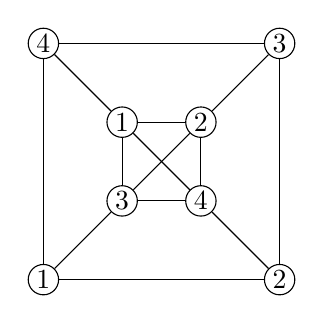
\begin{tikzpicture}
							\tikzstyle{vertex}=[circle,draw=black,minimum size=5pt,inner sep=1pt]
							\node[vertex] (1) at (0,0) {$4$};
							\node[vertex] (2) at (3,0) {$3$};
							\node[vertex] (3) at (0,-3) {$1$};
							\node[vertex] (4) at (3,-3) {$2$};
							\node[vertex] (5) at (1,-1) {$1$};
							\node[vertex] (6) at (2,-1) {$2$};
							\node[vertex] (7) at (1,-2) {$3$};
							\node[vertex] (8) at (2,-2) {$4$};
							\draw (1) -- (2);
							\draw (1) -- (3);
							\draw (1) -- (5);
							\draw (2) -- (4);
							\draw (2) -- (6);
							\draw (3) -- (4);
							\draw (3) -- (7);
							\draw (4) -- (8);
							\draw (5) -- (6);
							\draw (5) -- (7);
							\draw (5) -- (8);
							\draw (6) -- (7);
							\draw (6) -- (8);
							\draw (7) -- (8);
							\end{tikzpicture}
						\end{center}
					\end{proof}
				\subsection*{(b)}
					\textbf{Disprove}
					\begin{proof}
						下图(10.1的a图)存在如图所示的4染色方法:
						\begin{center}
							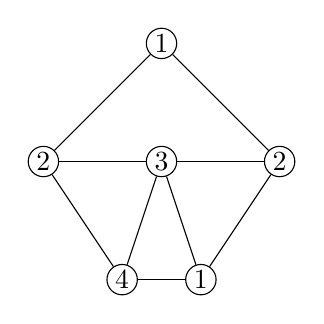
\begin{tikzpicture}
							\tikzstyle{vertex}=[circle,draw=black,minimum size=5pt,inner sep=1pt]
							\node[vertex] (1) at (0,0) {$1$};
							\node[vertex] (2) at (-1.5,-1.5) {$2$};
							\node[vertex] (3) at (0,-1.5) {$3$};
							\node[vertex] (4) at (1.5,-1.5) {$2$};
							\node[vertex] (5) at (-0.5,-3) {$4$};
							\node[vertex] (6) at (0.5,-3) {$1$};
							\draw (1) -- (2);
							\draw (1) -- (4);
							\draw (2) -- (3);
							\draw (3) -- (4);
							\draw (2) -- (5);
							\draw (3) -- (5);
							\draw (3) -- (6);
							\draw (4) -- (6);
							\draw (5) -- (6);
							\end{tikzpicture}
						\end{center}
						而在10.1中已证其色数为3,因此命题不正确.
					\end{proof}
				\subsection*{(c)}
					\textbf{Disprove}
					\begin{proof}
						如图:
						\begin{center}
							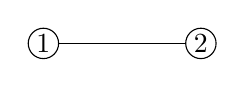
\begin{tikzpicture}
							\tikzstyle{vertex}=[circle,draw=black,minimum size=5pt,inner sep=1pt]
							\node[vertex] (1) at (0,0) {$1$};
							\node[vertex] (2) at (2,0) {$2$};
							\draw (1) -- (2);
							\end{tikzpicture}
						\end{center}
						该图只有两个顶点,没有染色数为3的情形,但$\chi(G)=2$.
					\end{proof}
				\subsection*{(d)}
					\textbf{Disprove}
					\begin{proof}
						$\chi(K_{3,3})=2$,而$K_{3,3}$不是平面图.
					\end{proof}
			\section*{10.10}
				将每一个课程作为图$G$中的顶点.顶点$v_1$与顶点$v_2$相邻当且仅当有一个学生同时修读了它们.由此,可如下构造:
				\begin{center}
					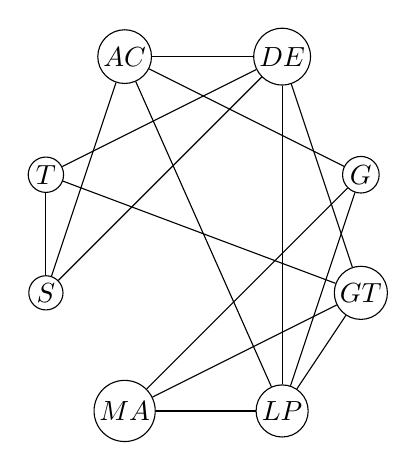
\begin{tikzpicture}
					\tikzstyle{vertex}=[circle,draw=black,minimum size=5pt,inner sep=1pt]
					\node[vertex] (1) at (0,0) {$AC$};
					\node[vertex] (2) at (2,0) {$DE$};
					\node[vertex] (3) at (3,-1.5) {$G$};
					\node[vertex] (4) at (3,-3) {$GT$};
					\node[vertex] (5) at (2,-4.5) {$LP$};
					\node[vertex] (6) at (0,-4.5) {$MA$};
					\node[vertex] (7) at (-1,-3) {$S$};
					\node[vertex] (8) at (-1,-1.5) {$T$};
					\draw (1) -- (2);
					\draw (1) -- (3);
					\draw (1) -- (5);
					\draw (1) -- (7);
					\draw (2) -- (4);
					\draw (2) -- (5);
					\draw (2) -- (7);
					\draw (2) -- (8);
					\draw (3) -- (5);
					\draw (3) -- (6);
					\draw (4) -- (5);
					\draw (4) -- (6);
					\draw (4) -- (8);
					\draw (5) -- (6);
					\draw (7) -- (8);		
					\end{tikzpicture}
				\end{center}
				因为包含三角形,所以$\chi(G)\ge3$,再证明$\chi(G)\neq3$:若$DE=1,LP=2$,则$GT=3$,则$MA=1$,则$G=3$,此时$AC$无法取1~3中的值,故$\chi(G)>3$.下面给出染色数为4的情形:
				\begin{center}
					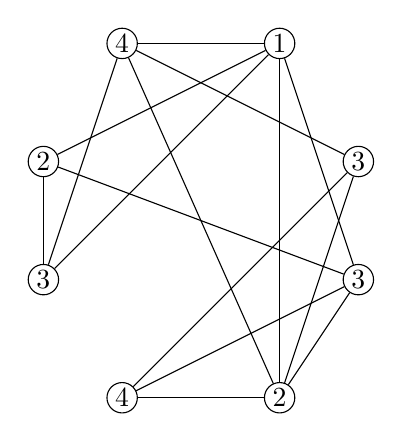
\begin{tikzpicture}
					\tikzstyle{vertex}=[circle,draw=black,minimum size=5pt,inner sep=1pt]
					\node[vertex] (1) at (0,0) {$4$};
					\node[vertex] (2) at (2,0) {$1$};
					\node[vertex] (3) at (3,-1.5) {$3$};
					\node[vertex] (4) at (3,-3) {$3$};
					\node[vertex] (5) at (2,-4.5) {$2$};
					\node[vertex] (6) at (0,-4.5) {$4$};
					\node[vertex] (7) at (-1,-3) {$3$};
					\node[vertex] (8) at (-1,-1.5) {$2$};
					\draw (1) -- (2);
					\draw (1) -- (3);
					\draw (1) -- (5);
					\draw (1) -- (7);
					\draw (2) -- (4);
					\draw (2) -- (5);
					\draw (2) -- (7);
					\draw (2) -- (8);
					\draw (3) -- (5);
					\draw (3) -- (6);
					\draw (4) -- (5);
					\draw (4) -- (6);
					\draw (4) -- (8);
					\draw (5) -- (6);
					\draw (7) -- (8);		
					\end{tikzpicture}
				\end{center}
				因此只需要4个不同时间段即可,也即最早结束时间为2:45-4:45.
			\section*{10.11}
				将每一种化学药品作为图$G$中的顶点,边$(v_1,v_2)$存在当且仅当$v_1$与$v_2$相互作用.于是可如下构造:
				\begin{center}
					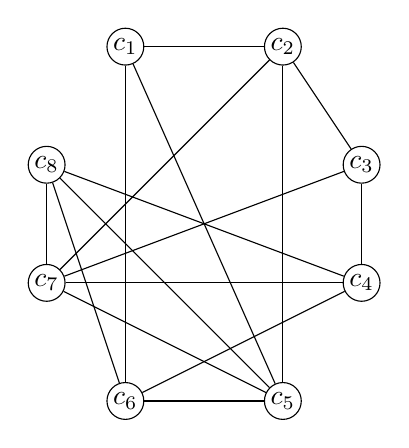
\begin{tikzpicture}
					\tikzstyle{vertex}=[circle,draw=black,minimum size=5pt,inner sep=1pt]
					\node[vertex] (1) at (0,0) {$c_1$};
					\node[vertex] (2) at (2,0) {$c_2$};
					\node[vertex] (3) at (3,-1.5) {$c_3$};
					\node[vertex] (4) at (3,-3) {$c_4$};
					\node[vertex] (5) at (2,-4.5) {$c_5$};
					\node[vertex] (6) at (0,-4.5) {$c_6$};
					\node[vertex] (7) at (-1,-3) {$c_7$};
					\node[vertex] (8) at (-1,-1.5) {$c_8$};
					\draw (1) -- (2);
					\draw (1) -- (5);
					\draw (1) -- (6);
					\draw (2) -- (3);
					\draw (2) -- (5);
					\draw (2) -- (7);
					\draw (3) -- (4);
					\draw (3) -- (7);
					\draw (4) -- (6);
					\draw (4) -- (7);
					\draw (4) -- (8);
					\draw (5) -- (6);
					\draw (5) -- (7);
					\draw (5) -- (8);
					\draw (6) -- (8);
					\draw (7) -- (8);		
					\end{tikzpicture}
				\end{center}
				因为包含三角形,所以$\chi(G)\ge3$.再证明$\chi(G)\neq3$:若$c_7=1,c_8=2$,则$c_4=3,c_3=2,c_2=3,c_5=2$.此时$c_8=c_5=2$,矛盾.因此$\chi(G)\ge4$.下面给出染色数为4的情形:
				\begin{center}
					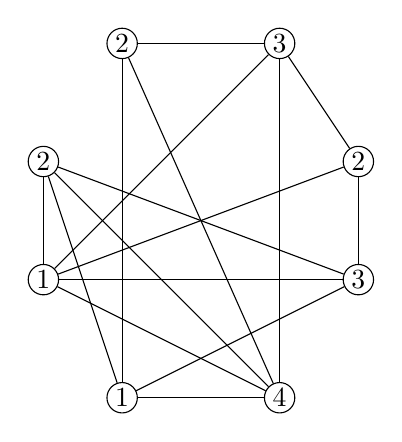
\begin{tikzpicture}
					\tikzstyle{vertex}=[circle,draw=black,minimum size=5pt,inner sep=1pt]
					\node[vertex] (1) at (0,0) {$2$};
					\node[vertex] (2) at (2,0) {$3$};
					\node[vertex] (3) at (3,-1.5) {$2$};
					\node[vertex] (4) at (3,-3) {$3$};
					\node[vertex] (5) at (2,-4.5) {$4$};
					\node[vertex] (6) at (0,-4.5) {$1$};
					\node[vertex] (7) at (-1,-3) {$1$};
					\node[vertex] (8) at (-1,-1.5) {$2$};
					\draw (1) -- (2);
					\draw (1) -- (5);
					\draw (1) -- (6);
					\draw (2) -- (3);
					\draw (2) -- (5);
					\draw (2) -- (7);
					\draw (3) -- (4);
					\draw (3) -- (7);
					\draw (4) -- (6);
					\draw (4) -- (7);
					\draw (4) -- (8);
					\draw (5) -- (6);
					\draw (5) -- (7);
					\draw (5) -- (8);
					\draw (6) -- (8);
					\draw (7) -- (8);		
					\end{tikzpicture}
				\end{center}
				因此至少需要4个容器,最小成本为380,容器1:$v_6,v_7$;容器2:$v_1,v_3,v_8$;容器3:$v_2,v_4$;容器4:$v_5$.
		\end{SChinese}
	\end{CJK}
\end{document}